\documentclass{article}
\usepackage{amsmath}
\usepackage{amssymb}
\usepackage[a4paper, top=25mm, bottom=25mm, left=25mm, right=25mm]{geometry}
\usepackage{pgfplots}
\usepackage{mathtools}
\usepackage{parskip}
\usepgfplotslibrary{fillbetween}
\pgfplotsset{compat=1.18}

\begin{document}
\pagestyle{empty}
\large

\begin{center}
\textbf{2015-2016 Fall \\MAT123 Final\\(12/01/2016)}
\end{center}

\textbf{1.} Find the area of the region bounded by the circle $x^2+y^2=1$ and the graph of the absolute value function $y=\left|x\right|$.

\vspace{1em}

\textbf{2.} Use the Washer Method to find the volume of the solid obtained by revolving the region bounded by the parabola $y=2x^2-3$ and the curves $y=-3,\:x=2$ about the line $y=7$.

\vspace{1em}

\textbf{3.} Use the Cylindrical Shell Method to find the volume of the solid obtained by revolving the region bounded by $y=x^2$ and $y=-x+1$ about the line $x=-1$.

\vspace{1em}

\textbf{4.} Evaluate the following integrals.

\textbf{(a)} $\displaystyle\int\frac{\sin \sqrt x}{\sqrt x}\,dx$

\textbf{(b)} $\displaystyle\int\frac{x^5+x^4-8x^3+10x^2+12x}{x^2-3x+2}\,dx$

\textbf{(c)} $\displaystyle\int\arccos x\,dx$

\textbf{(d)} $\displaystyle\int\frac1{x^2+3x+1}\,dx$

\textbf{(e)} $\displaystyle\int\frac{\sin x}{1+\sin x}\,dx$

\vspace{1em}

\textbf{5.} Find the surface area of the revolution by rotating the curve $y= e^x,\:0\leq x\leq1$ about the $x$-axis.

\vspace{1em}

\textbf{6.} Investigate the convergence of the improper integral $\displaystyle\int_0^{-\infty}\frac{ e^{-x}}{1+ e^{-x}}\,dx$.

\vspace{1em}

\textbf{7.} Using the Monotone Convergence Theorem, investigate the convergence of the sequence $\displaystyle\left(\frac{\ln n}n\right)_{n\in\mathbb{N}}$.

\newpage

\begin{center}
\textbf{2015-2016 Final (12/01/2016) Solutions\\
(Last update: 30/08/2025 00:48)}
\end{center}

\textbf{1.}
\begin{center}
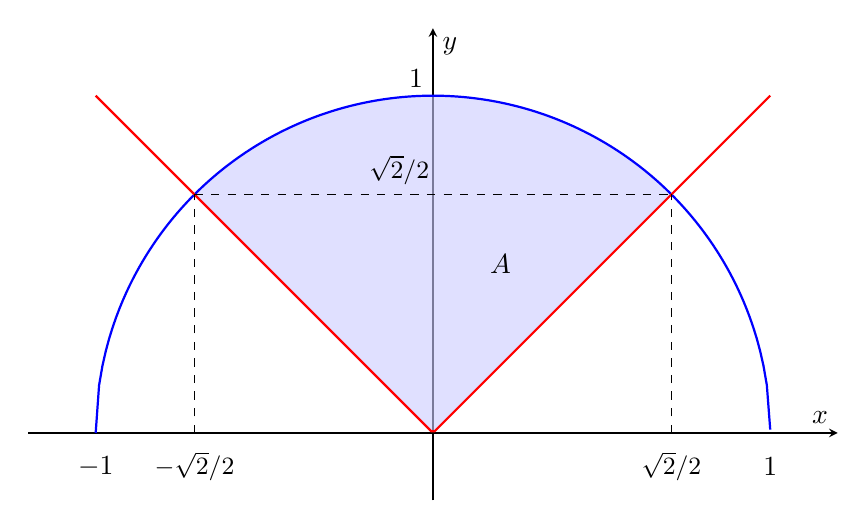
\begin{tikzpicture}
  \begin{axis}[
      axis lines=center,
      axis equal image,
      xlabel={$x$},
      ylabel={$y$},
      xtick=\empty, ytick=\empty,
      xmin=-1.2, xmax=1.2,
      ymin=-0.2, ymax=1.2,
      samples=200,
      scale=1.5,
      domain=-1:1,
    ]

    \addplot [thick, blue, name path=A, domain=-1:1] {sqrt(1-x^2)};
    \addplot [thick, red, name path=B] {abs(x)};
    \addplot [blue!20, fill opacity=0.6] fill between[of=A and B,soft clip={domain=-0.707:0.707}];
    
    \draw[dashed] (-0.707,0) -- (-0.707,0.707);
    \draw[dashed] (0.707,0) -- (0.707,0.707);
    \draw[dashed] (-0.707,0.707) -- (0.707,0.707);

    \node at (axis cs:0.707,-0.1) {\small $\sqrt2/2$};
    \node at (axis cs:-0.707,-0.1) {\small $-\sqrt2/2$};
    \node at (axis cs:-0.1,0.78) {\small $\sqrt2/2$};
    \node at (axis cs:-1,-0.1) {$-1$};
    \node at (axis cs:1,-0.1) {$1$};
    \node at (axis cs:-0.05,1.05) {$1$};
    \node at (0.2,0.5) {$A$};
\end{axis}
\end{tikzpicture}
\end{center}
\begin{align}
A&=\int_{-\sqrt2/2}^{\sqrt2/2}\left(\sqrt{1-x^2}-\left|x\right|\right)\,dx=\int_{-\sqrt2/2}^0\left(\sqrt{1-x^2}+x\right)\,dx+\int_0^{\sqrt2/2}\left(\sqrt{1-x^2}-x\right)\,dx\nonumber\\\nonumber\\&=\int_{-\sqrt2/2}^{\sqrt2/2}\sqrt{1-x^2}\,dx-\int_0^{\sqrt2/2}2x\,dx
\end{align}

Calculate the right-hand integral $(1)$.

\[\int_0^{\sqrt2/2}2x\,dx=x^2\bigg|_0^{\sqrt2/2}=\left(\frac{\sqrt2}2\right)^2-\left(0\right)^2=\frac12\]

To calculate the left-hand integral in $(1)$, we will use a trigonometric substitution. Let $x=\sin u$, then $dx=\cos u\,du$.

\[x=-\frac{\sqrt2}2\implies u=\arcsin\left(-\frac{\sqrt2}2\right)=-\frac{\pi}4,\qquad x=\frac{\sqrt2}2\implies u=\arcsin\left(\frac{\sqrt2}2\right)=\frac{\pi}4\]

\begin{align*}\int_{-\sqrt2/2}^{\sqrt2/2}\sqrt{1-x^2}\,dx&=\int_{-\pi/4}^{\pi/4}\sqrt{1-\sin^2u}\cos u\,du=\int_{-\pi/4}^{\pi/4}\left|\cos u\right|\cos u\,du\quad\left[\left|\cos u\right|>0\right]\\\\&=\int_{-\pi/4}^{\pi/4}\cos^2u\,du=\int_{-\pi/4}^{\pi/4}\frac{1+\cos2u}{2}\,du=\left[\frac u2+\frac{\sin2u}4\right]_{-\pi/4}^{\pi/4}\\\\&=\left(\frac\pi8+\frac14\right)-\left(-\frac\pi8-\frac14\right)=\frac\pi4-\frac12\end{align*}

Evaluate $(1)$. The area is $\displaystyle A=\left(\frac\pi4+\frac12\right)-\left(\frac12\right)=\boxed{\frac\pi4}$.

\newpage

\textbf{2.}
\begin{center}
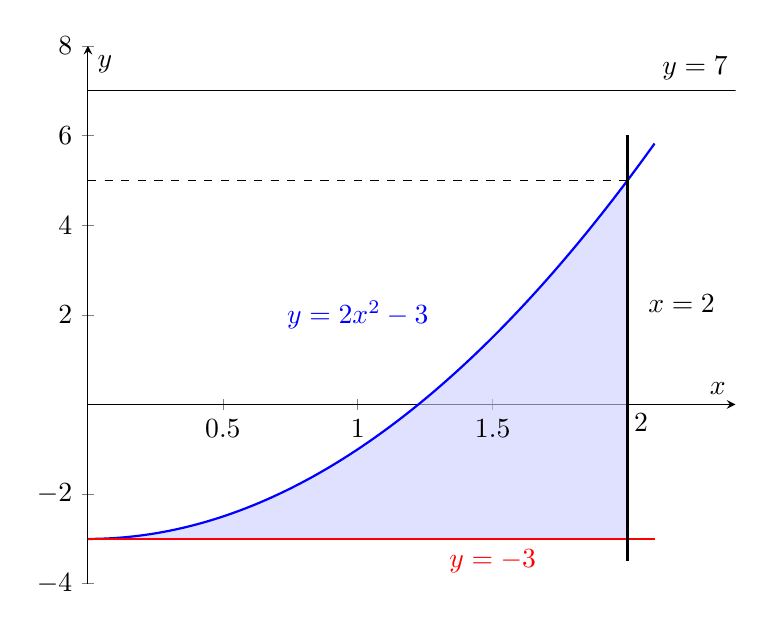
\begin{tikzpicture}
  \begin{axis}[
      axis lines=center,
      xlabel={$x$},
      ylabel={$y$},
      xmin=0, xmax=2.4,
      ymin=-4, ymax=8,
      samples=150,
      xticklabels={,,$0.5$,$1$,$1.5$,},
      clip=true,
      scale=1.2,
      domain=0:2.1,
    ]

    \addplot [thick, blue, name path=A] {2*x^2-3};
    \addplot [thick, red, name path=B] {-3};
    \addplot [blue!20, fill opacity=0.6] fill between[of=A and B,soft clip={domain=0:2}];
    \draw (0,7)--(5,7); \draw[thick] (2,-3.5)--(2,6); \draw[dashed] (0,5)--(2,5);
    \node at (2.25,7.5) {$y=7$};
    \node[blue] at (1,2) {$y=2x^2-3$};
    \node at (2.2,2.25) {$x=2$};
    \node[red] at (1.5,-3.5) {$y=-3$};
    \node at (2.05,-0.4) {$2$};
  \end{axis}
\end{tikzpicture}
\end{center}
\begin{align*}
V&=\int_D\pi\left[R_2^2(x)-R_1^2(x)\right]\,dx=\int_0^2\pi\left[\left(7-(-3)\right)^2-\left(7-\left(2x^2-3\right)\right)^2\right]\,dx\\\\&=\pi\int_0^2\left[(10)^2-\left(10-2x^2\right)^2\right]\,dx=\pi\int_0^2\left(100-100+40x^2-4x^4\right)\,dx\\\\&=\pi\int_0^2\left(40x^2-4x^4\right)\,dx=\pi\left[\frac{40x^3}3-\frac{4x^5}5\right]_0^2=\pi\left[\left(\frac{320}3-\frac{128}5\right)-\left(0\right)\right]=\boxed{\frac{1216\pi}{15}}
\end{align*}

\vspace{1em}

\textbf{3.}
\begin{center}
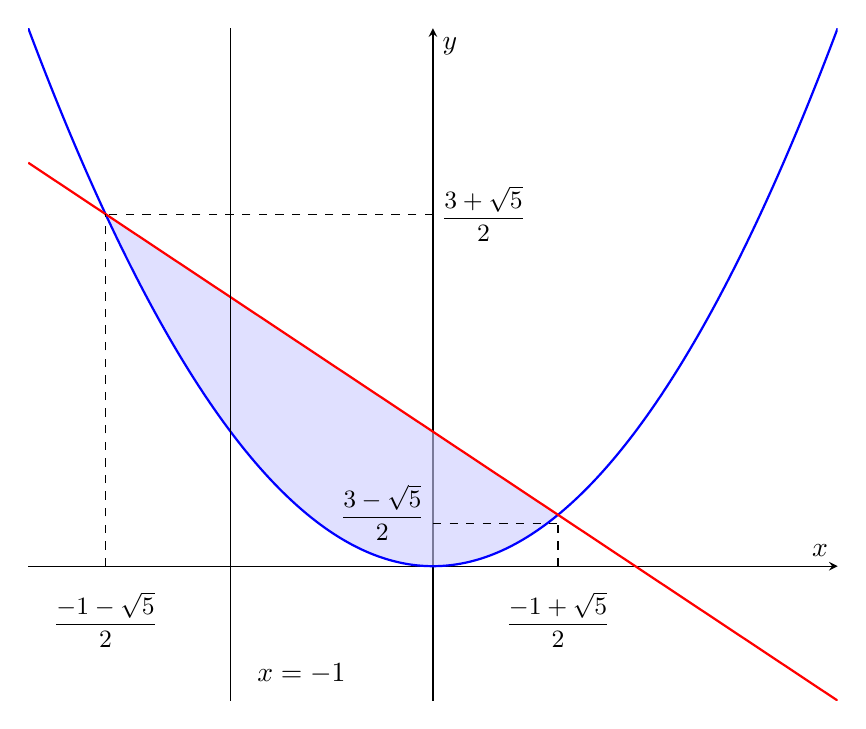
\begin{tikzpicture}
  \begin{axis}[
      axis lines=center,
      xlabel={$x$},
      ylabel={$y$},
      ytick=\empty, xtick=\empty,
      xmin=-2, xmax=2,
      ymin=-1, ymax=4,
      samples=250,
      clip=true,
      scale=1.5,
      domain=-2:2,
    ]

    \addplot [thick, blue, name path=A] {x^2};
    \addplot [thick, red, name path=B] {-x+1};
    \addplot [blue!20, fill opacity=0.6] fill between[of=A and B, soft clip={domain=-1.618:0.618}];
    
    \node at (-1.618,-0.4) {\small $\displaystyle\frac{-1-\sqrt5}2$};
    \node at (0.618,-0.4) {\small $\displaystyle\frac{-1+\sqrt5}2$};
    \node at (0.25,2.618) {\small $\displaystyle\frac{3+\sqrt5}2$};
    \node at (-0.25,0.4) {\small $\displaystyle\frac{3-\sqrt5}2$};
    \node at (-0.65,-0.8) {$x=-1$};
    
    \draw[dashed] (-1.618,0)--(-1.618,2.618); \draw[dashed] (0,2.618)--(-1.618,2.618);
    \draw[dashed] (0.618,0)--(0.618,0.318); \draw[dashed] (0,0.318)--(0.618,0.318);
    \draw (-1,-1)--(-1,4);
  \end{axis}
\end{tikzpicture}
\end{center}

Notice that the rotation axis passes through the region. Consider the right-hand region. If we rotate it around the axis, a piece of the region on the left will be inside the revolution. That is, the region bounded by the line that is symmetric to the line $y=-x+1$ around $x=-1$ and the curve $y=x^2$. We do not need to rotate that region since it would lead to double revolution. The upper part of the left-hand region may be rotated around $x=-1$ independent of the right-hand region. Divide the left-hand region into three subregions. We get three different subregions to integrate over.

\begin{center}
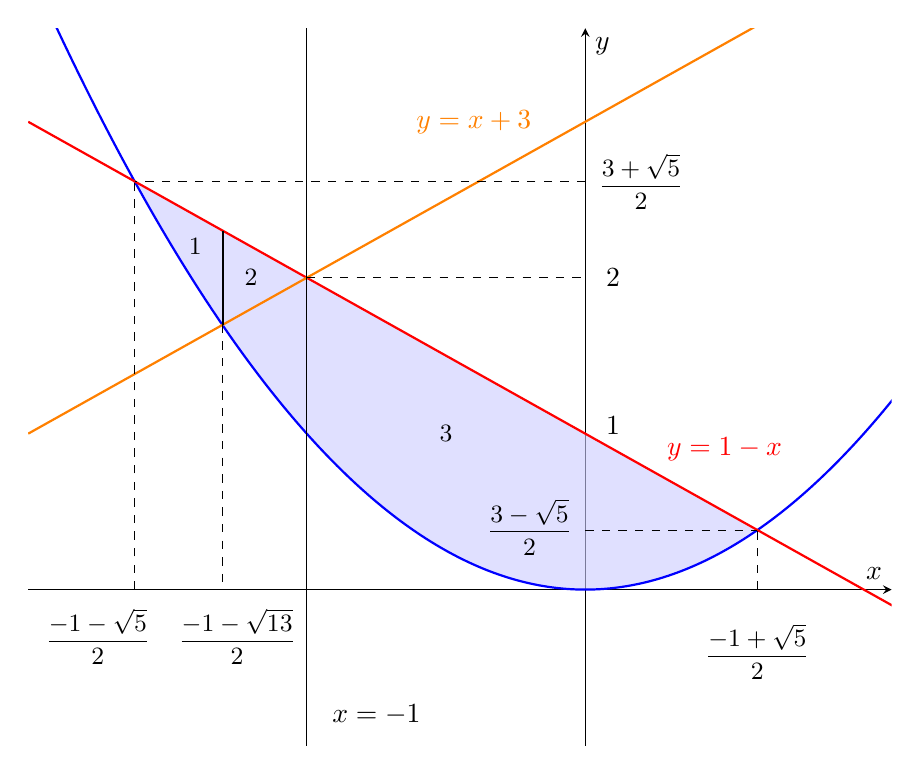
\begin{tikzpicture}
  \begin{axis}[
      axis lines=center,
      xlabel={$x$},
      ylabel={$y$},
      ytick=\empty, xtick=\empty,
      xmin=-2, xmax=1.1,
      ymin=-1, ymax=3.6,
      samples=250,
      clip=true,
      scale=1.6,
      domain=-2:2,
    ]

    \addplot [thick, blue, name path=A] {x^2};
    \addplot [thick, red, name path=B] {-x+1};
    \addplot [thick, orange] {x+3};
    \addplot [blue!20, fill opacity=0.6] fill between[of=A and B, soft clip={domain=-1.618:0.618}];
    
    \node at (-1.75,-0.3) {\small $\displaystyle\frac{-1-\sqrt5}2$};
    \node at (-1.25,-0.3) {\small $\displaystyle\frac{-1-\sqrt{13}}2$};
    \node at (0.618,-0.4) {\small $\displaystyle\frac{-1+\sqrt5}2$};
    \node at (0.2,2.618) {\small $\displaystyle\frac{3+\sqrt5}2$};
    \node at (-0.2,0.4) {\small $\displaystyle\frac{3-\sqrt5}2$};
    \node at (-0.75,-0.8) {$x=-1$};
    \node[orange] at (-0.4,3) {$y=x+3$};
    \node[red] at (0.5,0.9) {$y=1-x$};
    \node at (0.1,2) {$2$};
    \node at (0.1,1.05) {$1$};

    \draw[dashed] (-1.618,0)--(-1.618,2.618); \draw[dashed] (0,2.618)--(-1.618,2.618);
    \draw[dashed] (0.618,0)--(0.618,0.381); \draw[dashed] (0,0.381)--(0.618,0.381);
    \draw[thick] (-1.302, 1.698)--(-1.302,2.302);
    \draw[dashed] (-1.302, 1.698)--(-1.302,0);
    \draw[dashed] (-1,2)--(0,2);

    \node at (-1.4,2.2) {\small $1$};
    \node at (-1.2,2) {\small $2$};
    \node at (-0.5,1) {\small $3$};

    \draw (-1,-1)--(-1,4);
  \end{axis}
\end{tikzpicture}
\end{center}

Let $V$ be the volume of the solid.
\begin{align*}V&=\int_D2\pi\cdot r(x)\cdot h(x)\,dx\\\\&=\int_{\textstyle\frac{-1-\sqrt5}2}^{\textstyle\frac{1-\sqrt{13}}2}2\pi(-1-x)\left[\left(1-x\right)-x^2\right]\,dx+\int_{\textstyle\frac{1-\sqrt{13}}2}^{-1}2\pi(-1-x)\left[\left(1-x\right)-\left(x+3\right)\right]\,dx\\\\&\quad\:+\int_{-1}^{\textstyle\frac{-1+\sqrt5}2}2\pi\left(x+1\right)\left[\left(1-x\right)-x^2\right]\,dx\\\\&=2\pi\int_{\textstyle\frac{-1-\sqrt5}2}^{\textstyle\frac{1-\sqrt{13}}2}\left(-1+2x^2+x^3\right)\,dx+2\pi\int_{\textstyle\frac{1-\sqrt{13}}2}^{-1}\left(2x^2+4x+2\right)\,dx\\\\&\quad\:+2\pi\int_{-1}^{\textstyle\frac{-1+\sqrt5}2}\left(1-2x^2-x^3\right)\,dx\\\\&=2\pi\left\{\left[-x+\frac{2x^3}3+\frac{x^4}4\right]_{\textstyle\frac{-1-\sqrt5}2}^{\textstyle\frac{1-\sqrt{13}}2}+\left[\frac{2x^3}3+2x^2+2x\right]_{\textstyle\frac{1-\sqrt{13}}2}^{-1}+\left[x-\frac{2x^3}3-\frac{x^4}4\right]_{-1}^{\textstyle\frac{-1+\sqrt5}2}\right\}\end{align*}

\newpage

\begin{align*}V&=2\pi\left[\frac{\sqrt{13}-1}2+\frac{\left(1-\sqrt{13}\right)^3}{12}+\frac{\left(1-\sqrt{13}\right)^4}{64}-\frac{1+\sqrt5}2+\frac{\left(1+\sqrt5\right)^3}{12}-\frac{\left(1+\sqrt5\right)^4}{64}\right]\\\\&\quad\:+2\pi\left[-\frac23+2-2-\left(\frac{\left(1-\sqrt{13}\right)^3}{12}+\frac{\left(1-\sqrt{13}\right)^2}2+1-\sqrt{13}\right)\right]\\\\&\quad\:+2\pi\left[\frac{-1+\sqrt5}2-\frac{\left(-1+\sqrt5\right)^3}{12}-\frac{\left(-1+\sqrt5\right)^4}{64}-\left(-1+\frac23-\frac14\right)\right]\end{align*}

After some mathematical operations, the volume is found to be

\[V=\frac{13\pi}6-\frac{\pi}4\left(47-13\sqrt{13}\right)=\boxed{\frac{\pi\left(39\sqrt{13}-115\right)}{12}}\]

The volume can also be evaluated by integrating over the domain and subtracting the region that is revolved twice. That is, the region beneath the region $2$ mapped on the graph.

\vspace{1em}

\textbf{4. (a)} Let $u=\sqrt x$, then $\displaystyle du=\frac1{2\sqrt x}\,dx$.
\[\int\frac{\sin\sqrt x}{\sqrt x}\,dx=\int\sin u\cdot2\,du=-2\cos u+c=\boxed{-2\cos\sqrt x+c,\quad c\in\mathbb{R}}\]

\textbf{(b)} Perform a long polynomial division and rewrite the integral in two expressions.

\begin{align}I&=\int\frac{x^5+x^4-8x^3+10x^2+12x}{x^2-3x+2}\,dx=\int\left(x^3-4x^2-22x-48+\frac{-88x+96}{x^2-3x+2}\right)\,dx\nonumber\\\nonumber\\&=\int\left(x^3+4x^2+2x+8\right)\,dx+\int\frac{32x-16}{(x-2)(x-1)}\,dx\end{align}

Calculate the integral on the left in $(2)$.

\[\int\left(x^3+4x^2+2x+8\right)\,dx=\frac{x^4}4+\frac{4x^3}3+x^2+8x+c_1\]

Calculate the integral on the right in $(2)$. Decompose the expression into partial fractions.

\[\int\frac{32x-16}{(x-2)(x-1)}\,dx=\int\left(\frac{A}{x-2}+\frac{B}{x-1}\right)\,dx\]

\[32x-16=A(x-1)+B(x-2)=x(A+B)-A-2B\]

Equate the coefficients of like terms.

\[\left.\begin{array}{c}
A+B=32\\
-A-2B=-16 
\end{array}\right\}\rightarrow A=48,\quad B=-16\]

Substitute the values into $A$ and $B$.

\[\int\left(\frac{A}{x-2}+\frac{B}{x-1}\right)\,dx=\int\left(\frac{48}{x-2}-\frac{16}{x-1}\right)\,dx=48\ln|x-2|-16\ln|x-1|+c_2\]

Rewrite $(2)$.

\[I=\boxed{\frac{x^4}4+\frac{4x^3}3+x^2+8x+48\ln|x-2|-16\ln|x-1|+c,\quad c\in\mathbb{R}}\]

\textbf{(c)} Apply integration by parts.

\[\left.\begin{array}{c}
\displaystyle u=\arccos x\rightarrow du=-\frac1{\sqrt{1-x^2}}\,dx\\
\displaystyle dv=dx\rightarrow v=x
\end{array}\right\}\rightarrow\int v\,du=uv-\int v\,du\]

\[\int\arccos x\,dx=x\arccos x-\int\frac{-x}{\sqrt{1-x^2}}\,dx\]

Let us use a $u$-substitution for the integral on the right. Let $u=1-x^2$, then $du=-2x\,dx$

\[\int\frac{-x}{\sqrt{1-x^2}}\,dx=\int\frac{du}{2\sqrt u}=\sqrt u+c=\sqrt{1-x^2}+c\]

Therefore,

\[\int\arccos x\,dx=\boxed{x\arccos x-\sqrt{1-x^2}+c,\quad c\in\mathbb{R}}\]

\textbf{(d)} Use the method of partial fraction decomposition.

\begin{align*}I&=\int\frac{dx}{x^2+3x+1}=\int\frac{dx}{x^2+3x+\frac94-\frac54}=\int\frac{dx}{\left(x+\frac32\right)^2-\left(\frac{\sqrt5}2\right)^2}\\\\&=\int\frac{dx}{\left(x+\frac32-\frac{\sqrt5}2\right)\left(x+\frac32+\frac{\sqrt5}2\right)}=\int\left(\frac A{x+\frac32-\frac{\sqrt5}2}+\frac B{x+\frac32+\frac{\sqrt5}2}\right)\,dx\end{align*}

\[A\left(x+\frac32+\frac{\sqrt5}2\right)+B\left(x+\frac32-\frac{\sqrt5}2\right)=1\]
\[x(A+B)+A\left(\frac{3+\sqrt5}2\right)+B\left(\frac{3-\sqrt5}2\right)=1\]

Equate the coefficients of like terms.

\[\left.\begin{array}{c}
A+B=0\\
A\left(\frac{3+\sqrt5}2\right)+B\left(\frac{3-\sqrt5}2\right)=1
\end{array}\right\}\implies A=\frac1{\sqrt5},\quad B=-\frac1{\sqrt5}\]

Substitute the values into $A$ and $B$.
\begin{align*}I&=\int\left(\frac A{x+\frac32-\frac{\sqrt5}2}+\frac B{x+\frac32+\frac{\sqrt5}2}\right)\,dx\\\\&=\int\left(\frac1{\sqrt5\left(x+\frac32-\frac{\sqrt5}2\right)}-\frac1{\sqrt5\left(x+\frac32+\frac{\sqrt5}2\right)}\right)\,dx\\\\&=\boxed{\frac1{\sqrt5}\left(\ln\left|x+\frac32-\frac{\sqrt5}2\right|-\ln\left|x+\frac32+\frac{\sqrt5}2\right|\right)+c,\quad c\in\mathbb{R}}\end{align*}

\textbf{(e)}
\begin{align*}I=\int\frac{\sin x}{1+\sin x}\,dx=\int\frac{1+\sin x-1}{1+\sin x}\,dx=\int dx-\int\frac{dx}{1+\sin x}\end{align*}

The integral on the left evaluates to $x+c_1$. Evaluate the other integral.

\begin{align*}\int\frac{dx}{1+\sin x}&=\int\frac{1-\sin x}{(1+\sin x)(1-\sin x)}\,dx=\int\frac{1-\sin x}{1-\sin^2x}\,dx=\int\frac{1-\sin x}{\cos^2x}\,dx\\\\&=\int\left(\sec^2x-\tan x\sec x\right)\,dx=\tan x-\sec x+c_2\end{align*}

So, the result is
\[I=\boxed{x-\tan x+\sec x+c,\quad c\in\mathbb{R}}\]

\vspace{1em}

\textbf{5.} If the function $y=f(x)\geq0$ is continuously differentiable on $[a,b]$, the area of the surface generated by revolving the graph of $y=f(x)$ about the $x$-axis is

\[S=\int_a^b2\pi y\sqrt{1+\left(\frac{dy}{dx}\right)^2}\,dx\]
Find $\displaystyle\frac{dy}{dx}$.
\[\frac{dy}{dx}= e^x\]

Set $a=0$ and $b=1$ and then evaluate the integral.

\[S=\int_0^12\pi e^x\sqrt{1+\left( e^x\right)^2}\,dx\]

Let $u= e^x$, then $du= e^x\,dx$.

\[x=0\implies u= e^0=1,\qquad x=1\implies u= e^1= e\]

\[S=\int_0^12\pi e^x\sqrt{1+\left( e^x\right)^2}\,dx=2\pi\int_1^{ e}\sqrt{1+u^2}\,du\]

We will now use a trigonometric substitution. Let $u=\tan t$ for $\displaystyle0<t<\frac\pi2$, then $du=\sec^2 t\,dt$.
\begin{align*}S&=2\pi\int_1^{ e}\sqrt{1+u^2}\,du=2\pi\int\sqrt{1+\tan^2t}\cdot\sec^2t\,dt=2\pi\int\sqrt{\sec^2t}\cdot\sec^2t\,dt\\\\&=2\pi\int\left|\sec t\right|\sec^2t\,dt=2\pi\int\sec^3t\,dt\qquad\left[\sec t>0\right]\end{align*}

Find the antiderivative of $\sec^3t$ with the help of integration by parts.
\begin{align*}
    w=\sec t\,&\rightarrow\, dw = \sec t\tan t \,dt\\
    dz=\sec^2t\,dt\,&\rightarrow\, z = \tan t
\end{align*}
\begin{align*}
\int\sec^3t\,du&=\tan t\cdot\sec t-\int\tan^2 t\sec t\,dt=\tan t\cdot\sec t-\int\frac{1-\cos^2t}{\cos^3 t}\,dt\\\\&=\tan t\cdot\sec t-\int\sec^3t\,dt+\int\sec t\,dt 
\end{align*}

Notice that the integral appears on the right side of the equation. Therefore,

\[\int\sec^3t\,dt=\frac12\cdot\tan t\cdot\sec t+\frac12\cdot\int\sec t\,dt\]

The integral of $\sec t$ with respect to $t$ is

\[\int\sec t\,dt=\ln\left|\tan t+\sec t\right|+c_1,\quad c_1\in\mathbb{R}\]

Recall $u=\tan t$.
\[u=\tan t\implies u^2=\tan^2t=\sec^2t-1\implies \sec t=\sqrt{u^2+1}\]

\newpage

\begin{align*}S&=2\pi\cdot\frac12\left(\tan t\cdot\sec t+\ln\left|\tan t+\sec t\right|\right)+c=\pi\left[u\cdot\sqrt{u^2+1}+\ln\left|t+\sqrt{u^2+1}\right|\right]_1^{ e}\\\\&=\pi\left[\left( e\cdot\sqrt{ e^2+1}+\ln\left| e+\sqrt{ e^2+1}\right|\right)-\left(\sqrt2+\ln\left|1+\sqrt2\right|\right)\right]\\\\&=\boxed{\pi\left[ e\cdot\sqrt{ e^2+1}-\sqrt2+\ln\left(\frac{ e+\sqrt{ e^2+1}}{1+\sqrt2}\right)\right]}\end{align*}

\vspace{1em}

\textbf{6.} Let $u=1+ e^{-x}$, then $du=- e^{-x}\,dx$. Handle the improper integral by taking the limit.

\[x=0\implies u=1+ e^0=2,\qquad x\to-\infty\implies u\to\infty\]
\begin{align*}\int_0^{-\infty}\frac{ e^{-x}}{1+ e^{-x}}\,dx&=\int_2^{\infty}-\frac{du}{u}=\lim_{R\to\infty}\int_2^R-\frac{du}{u}=\lim_{R\to\infty}\left(-\ln u\right)\bigg|_2^R\\\\&=\lim_{R\to\infty}\left(-\ln R+\ln2\right)=\boxed{-\infty}\end{align*}

The integral diverges to negative infinity.

\vspace{1em}

\textbf{7.} According to the Monotone Convergence Theorem, if a sequence is both bounded and monotonic, the sequence converges. Take the corresponding function $\displaystyle f(x)=\frac{\ln x}x$. Apply the first derivative test and find the extrema.
\[f'(x)=\frac{\frac1x\cdot x-\ln x\cdot1}{x^2}=\frac{1-\ln x}{x^2}\]
\[f'(x)=0\implies 1-\ln x=0\implies \ln x=1\implies x= e\]

A critical point occurs at $x= e$. Apply the second derivative test and determine whether this is a local minimum or a local maximum.
\[f''(x)=\frac{-\frac1x\cdot x^2-(1-\ln x)\cdot 2x}{x^4}=\frac{2\ln x-3}{x^3}\]
\[f''( e)=\frac{-1}{ e^3}<0\]

Therefore, this is a local maximum.

The first term of the sequence is $\displaystyle\frac{\ln 1}1=0$. Take the limit at infinity. We may apply L'Hôpital's rule because we have an indeterminate form, which is $\infty/\infty$.

\[\lim_{x\to\infty}\frac{\ln x}{x}\overset{\text{L'H.}}{=}\lim_{x\to\infty}\frac{\frac1x}1=\lim_{x\to\infty}\frac1x=0\]

Since $\displaystyle\frac{\ln x}x$ is decreasing and bounded above by $\displaystyle f( e)=\frac1{ e}$ and below by $0$ for $x\geq e$, by the Monotone Convergence Theorem, the sequence converges.

\end{document}